% Compact trust-game exchange. Amounts are illustrative; explain in caption.
% Requires \usepackage{tikz}. Natural bounding box fits the exchange only.
\begingroup
\definecolor{TGink}{HTML}{242424}
\definecolor{TGline}{HTML}{989898}
\definecolor{TGfill}{HTML}{F5F5F3}
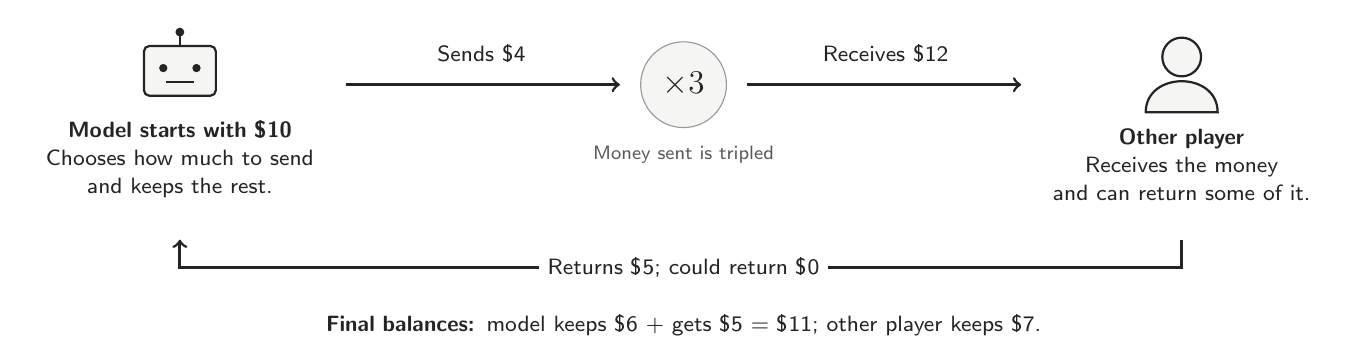
\begin{tikzpicture}[x=1pt,y=1pt,text=TGink,
  arrow/.style={->,draw=TGink,line width=1pt},
  textnode/.style={align=center,inner sep=0pt,font=\sffamily\fontsize{8}{10}\selectfont}]
  % Simple neutral icons; world colors are reserved for empirical plots.
  \draw[TGink,fill=TGfill,rounded corners=2pt,line width=.8pt] (39,-39) rectangle (65,-57);
  \draw[TGink,line width=.8pt] (52,-39) -- (52,-35);
  \fill[TGink] (52,-34) circle (1.6pt);
  \fill[TGink] (46,-47) circle (1.5pt);
  \fill[TGink] (58,-47) circle (1.5pt);
  \draw[TGink,line width=.7pt] (47,-52) -- (57,-52);
  \node[textnode,anchor=north,text width=110pt] at (52,-66)
    {\textbf{Model starts with \$10}\\Chooses how much to send\\and keeps the rest.};

  \draw[TGink,fill=TGfill,line width=.8pt] (414,-43) circle (7pt);
  \draw[TGink,fill=TGfill,line width=.8pt] (401,-63) .. controls (401,-48) and (427,-48) .. (427,-63) -- cycle;
  \node[textnode,anchor=north,text width=110pt] at (414,-69)
    {\textbf{Other player}\\Receives the money\\and can return some of it.};

  \draw[arrow] (112,-53) -- (211,-53);
  \node[textnode,anchor=south] at (161,-45) {Sends \$4};
  \node[textnode,draw=TGline,circle,fill=TGfill,minimum size=31pt,
    font=\sffamily\bfseries\fontsize{12}{14}\selectfont] at (234,-53) {$\times 3$};
  \draw[arrow] (257,-53) -- (356,-53);
  \node[textnode,anchor=south] at (307,-45) {Receives \$12};
  \node[textnode,anchor=north,text=black!65,font=\sffamily\fontsize{7}{9}\selectfont]
    at (234,-75) {Money sent is tripled};

  \draw[arrow] (414,-109) -- (414,-119) -- (52,-119) -- (52,-109);
  \node[textnode,fill=white,inner sep=3pt] at (234,-119)
    {Returns \$5; could return \$0};
  \node[textnode,anchor=north,text width=458pt] at (234,-136)
    {\textbf{Final balances:} model keeps \$6 + gets \$5 = \$11; other player keeps \$7.};
\end{tikzpicture}
\endgroup
